\documentclass[10pt,mathserif,aspectratio=169]{beamer}

\usepackage{graphicx,amsmath,amssymb,tikz,psfrag,booktabs,natbib,adjustbox}

\renewcommand{\familydefault}{\sfdefault}
\newcommand{\indep}{\perp\!\!\!\!\perp} % the independent symbol

% % define theorem
% \newtheorem{theorem}{Theorem}[section]
% \newtheorem{corollary}[theorem]{Corollary}
% \newtheorem{assumption}{Assumption}[subsection]
% % define definition style
% \theoremstyle{definition}
% \newtheorem{definition}{Definition}[section]
% \newtheorem{proposition}{Proposition}[section]
% \newtheorem{property}{Property}[section]
% \newtheorem{example}{Example}[section]
% \newtheorem*{exercise}{Exercise}
% % define remark style
% \theoremstyle{remark}
% \newtheorem*{remark}{Remark}
% \newtheorem{question}{Question}
% \newenvironment{sol}{\begin{proof}[Solution]}{\end{proof}}

\newcommand{\R}{\mathbb{R}}
\newcommand{\C}{\mathbb{C}}
\newcommand{\Rd}{\mathbb{R}^d}
\newcommand{\Hy}{\mathbb{H}}
\newcommand{\calh}{\mathcal{H}}
\newcommand{\cala}{\mathcal{A}}
\newcommand{\calm}{\mathcal{M}}
\newcommand{\cald}{\mathcal{D}}
\newcommand{\caln}{\mathcal{N}}
\newcommand{\calr}{\mathcal{R}}
\newcommand{\calz}{\mathcal{Z}}
\newcommand{\caly}{\mathcal{Y}}
\newcommand{\calq}{\mathcal{Q}}
\newcommand{\cale}{\mathcal{E}}
\newcommand{\cali}{\mathcal{I}}
\newcommand{\calb}{\mathcal{B}}
\newcommand{\calc}{\mathcal{C}}
\newcommand{\calw}{\mathcal{W}}
\newcommand{\calg}{\mathcal{G}}
\newcommand{\calu}{\mathcal{U}}
\newcommand{\calo}{\mathcal{O}}
\newcommand{\calp}{\mathcal{P}}
\newcommand{\vect}{\mathrm{vect}}
\newcommand{\cov}{\mathrm{cov}}
\newcommand{\reff}{\mathrm{ref}}

\newcommand{\setbra}[1]{\left\{#1\right\}}
\newcommand{\set}[1]{\setbra{#1}}
\newcommand{\bra}[1]{\left[#1\right]}
\newcommand{\pa}[1]{\left(#1\right)}
\newcommand{\abs}[1]{\left| #1\right|}
\newcommand{\norm}[1]{\left\| #1 \right\|}
\newcommand{\angs}[1]{\left\langle #1\right\rangle}
\newcommand{\midvert}{\middle|}

\newcommand{\Q}{\mathbb{Q}}
\newcommand{\Lip}{\mathrm{Lip}}
\newcommand{\Z}{\mathbb{Z}}
\newcommand{\N}{\mathbb{N}}
\newcommand{\Cpx}{\mathbb{C}}
\newcommand{\E}{\mathbb{E}}
\newcommand{\V}{\mathbb{V}}
\newcommand{\Var}{\mathrm{Var}}
\newcommand{\p}{\mathbb{P}}
\newcommand{\F}{\mathcal{F}}
%\newcommand{\G}{\mathcal{G}}
\newcommand{\diag}{\mathrm{diag}}
\newcommand{\id}{\mathrm{id}}
\newcommand{\one}{\mathbbm{1}}
\newcommand{\defeq}{\overset{\mathrm{def}}{=}}
\newcommand{\nlr}{\nleftrightarrow}
\newcommand{\lr}{\leftrightarrow}
\newcommand{\ra}{\rightarrow}
\newcommand{\tr}{\mathrm{tr}}
\newcommand{\pspace}{(\Omega, \F, \p)}
\newcommand{\filt}{\pa{\F_t}_{0\leq t\leq \infty}}
\newcommand{\filtnat}{\pa{\F_t^X}_{0\leq t\leq \infty}}
\newcommand{\filtspace}{\pa{\Omega, \F, \filt, \p}}
\newcommand{\indist}[1]{\overset{d}{#1}}
\newcommand{\inlo}[1]{\overset{L^1}{#1}}
\newcommand{\inltwo}[1]{\overset{L^2}{#1}}
\newcommand{\inp}[1]{\overset{\p}{#1}}
\newcommand{\inpc}{\overset{\p}{\rightarrow}}
\newcommand{\indistc}{\indist{\rightarrow}}
\newcommand{\inas}[1]{\overset{\mathrm{a.s.}}{#1}}
\newcommand{\inhy}[1]{\overset{\mathrm{\Hy^2}}{#1}}
\newcommand{\cc}[1]{\mathrm{CC}\left(#1 \right)}
\newcommand{\partfrac}[1]{\frac{\partial}{\partial #1}} \newcommand{\Chi}{\mathcal{X}} \newcommand{\tl}{{T,\Lambda}}
\newcommand{\isingspace}{\{\pm\}^\Lambda} \newcommand{\boltzmeas}{\mu_\tl}
\newcommand{\bl}{{\beta, \Lambda}} \newcommand{\zerot}{{t\in [0,T]}}
\newcommand{\tgez}{{t\geq 0}} \newcommand{\brown}{(B_t)_\tgez}
\newcommand{\process}{(X_t)_\tgez} \newcommand{\smallising}[4]{\begin{matrix} #1&#2\\#3&#4\end{matrix}}
\def\ci{\perp\!\!\!\!\perp}
\newcommand{\parm}{{(m)}} \newcommand{\diff}{\mathrm{d}} \newcommand{\optp}{\mathrm{opt}_\p}
\newcommand{\erp}{\mathrm{er}_\p} \newcommand{\er}{\mathrm{er}}
\newcommand{\sgn}{\mathrm{sgn}} \DeclareMathOperator*{\argmin}{arg\,min}
\DeclareMathOperator*{\argmax}{arg\,max}
\DeclareMathOperator*{\esssup}{ess\,sup}
\DeclareMathOperator*{\essinf}{ess\,inf} \newcommand{\vcdim}{\mathrm{VCdim}}
\newcommand{\bigargs}{\pa{\bar{Y}_t,M_t,\theta_t}}
\newcommand{\bigargsm}{\pa{\bar{Y}_{t-},M_{t-},\theta_{t-}}}
\newcommand{\smallargs}{\pa{\bar{y},m,\vartheta}}
\newcommand{\smallarg}{\pa{m,\vartheta}}

\newcommand{\fatone}{\mathbf{1}}
\newcommand{\pen}{\mathrm{pen}}
\newcommand{\MF}{\mathrm{MF}}
\newcommand{\opt}{\mathrm{opt}}
\newcommand{\MSE}{\mathrm{MSE}}
\newcommand{\MISE}{\mathrm{MISE}}
\newcommand{\CV}{\mathrm{CV}}

\newcommand{\1}{\mathbbm{1}}



%% striketrough
\usepackage[normalem]{ulem}
\renewcommand{\footnotesize}{\scriptsize}
%% formatting

\mode<presentation>
{
  \usetheme{default}
}
\setbeamertemplate{navigation symbols}{}
\usecolortheme[rgb={0.13,0.28,0.59}]{structure}
\definecolor{darkblue}{rgb}{0.13,0.28,0.59}
\definecolor{brilliantrosy}{RGB}{242,65,169}
\setbeamercolor{alerted text}{fg=darkblue}
\setbeamertemplate{itemize subitem}{--}
\setbeamertemplate{frametitle} {
  \begin{center}
    {\large\bf \insertframetitle}
  \end{center}
}

\newcommand\footlineon{
  \setbeamertemplate{footline} {
    \begin{beamercolorbox}[ht=2.5ex,dp=1.125ex,leftskip=.8cm,rightskip=.6cm]{structure}
      \footnotesize \insertsection
      \hfill
      {\insertframenumber}
    \end{beamercolorbox}
    \vskip 0.45cm
  }
}
\footlineon

% backup slides
\usepackage{appendixnumberbeamer}
\newcommand{\beginbackup}{
  \newcounter{framenumbervorappendix}
  \setcounter{framenumbervorappendix}{\value{framenumber}}
  \setbeamertemplate{footline}
  {
    \leavevmode%
    \hline
    box{%
        \begin{beamercolorbox}[wd=\paperwidth,ht=2.25ex,dp=1ex,right]{footlinecolor}%
          %         \insertframenumber  \hspace*{2ex} 
        \end{beamercolorbox}}%
    \vskip0pt%
  }
}
\newcommand{\backupend}{
  \addtocounter{framenumbervorappendix}{-\value{framenumber}}
  \addtocounter{framenumber}{\value{framenumbervorappendix}}
}

% \AtBeginSection[]
% {
%   \begin{frame}<beamer>
%     \frametitle{Outline}
%     \tableofcontents[currentsection,currentsubsection]
%   \end{frame}
% }

%% begin presentation

\title{\large \bfseries Return to \sout{Schooling} Holiday \\
  The potential impact of school holiday reform
}
\author{Fu Zixuan\\[3ex]
}
% }
\date{\today}
\titlegraphic{
\includegraphics[width=0.5\textwidth]{../Figures/vacances.jpg}}

\begin{document}

\frame{
  \thispagestyle{empty}
  \titlepage
}

% \section{Introduction}

\begin{frame}[label=motivation]
  \frametitle{Motivation}
  Last year when visiting a school in Marseille, Emmanuel Macron revived the
  debate on the school holiday, which he
  considers too long and believes increases inequalities between students from different financial backgrounds.

  \begin{itemize}
    \item What is the right length of school holiday, and what should we do with it?
    \item (Long) school holiday
          \begin{itemize}
            \item cons: summer learning loss (+ crammed school day), increase in social
                  inequalities, working parents.
            \item pros: for obvious reasons (who doesn't like holidays?)
          \end{itemize}
    \item Potential reform
          \begin{itemize}
            \item Rearrange the school calendar, e.g., shorten the summer holiday.
            \item \textit{"Vacances apprenantes"} initiatives (learning holidays).
          \end{itemize}
  \end{itemize}
\end{frame}

\begin{frame}[label=background1]
  \frametitle{Background: Length of holiday across Europe}
  The data is from \href{https://op.europa.eu/en/publication-detail/-/publication/080f40cc-63d3-11ed-92ed-01aa75ed71a1/language-en/format-PDF/source-275370246}{Eurydice}, visualized by \href{https://www.lemonde.fr/les-decodeurs/article/2023/08/29/rythmes-scolaires-la-france-a-t-elle-les-plus-longues-vacances-en-europe_6186976_4355770.html}{lemonde.fr}\footnote{Data not available for Germany, Spain, and Switzerland due to variations between federal states (Germany), autonomous regions (Spain), or cantons (Switzerland).}
  \begin{columns}[T,onlytextwidth]
    \column{0.5\textwidth}
    Overall holiday:
    \begin{figure}
      \centering
      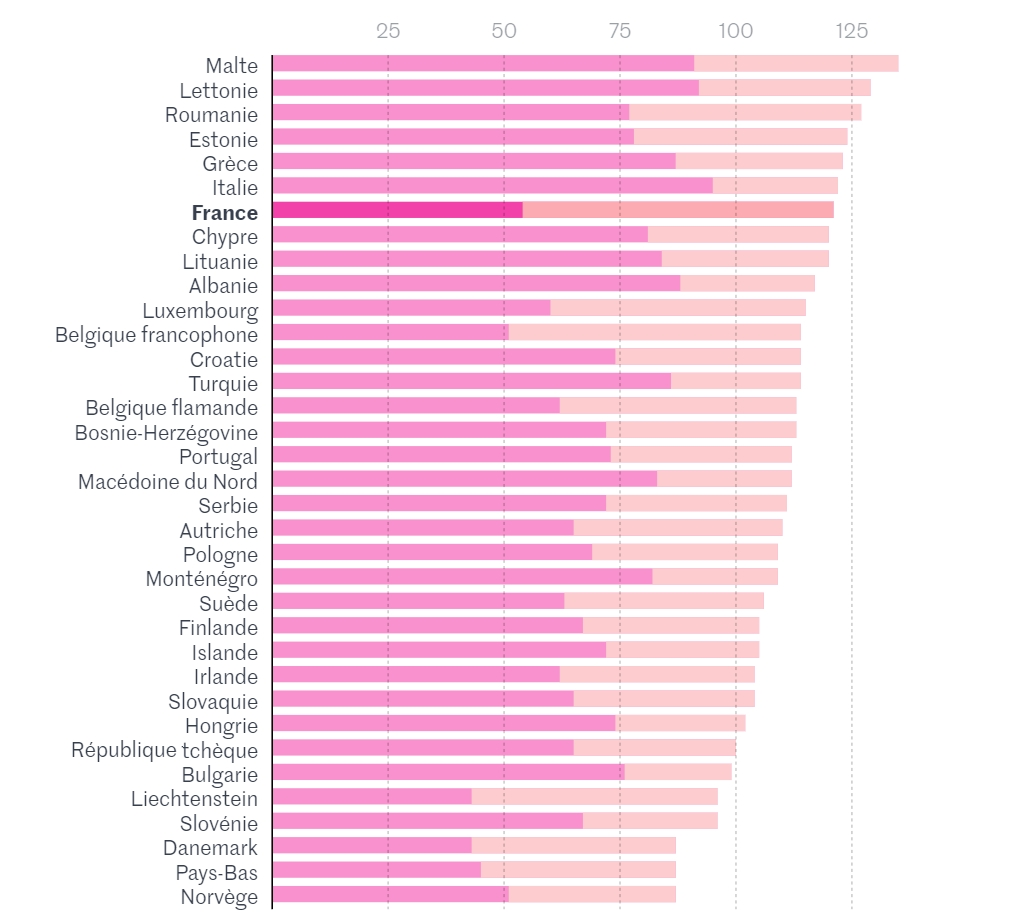
\includegraphics[width=0.9\textwidth]{../Figures/holiday_all.png}
    \end{figure}

    \column{0.5\textwidth}
    Small holiday:
    \begin{figure}
      \centering
      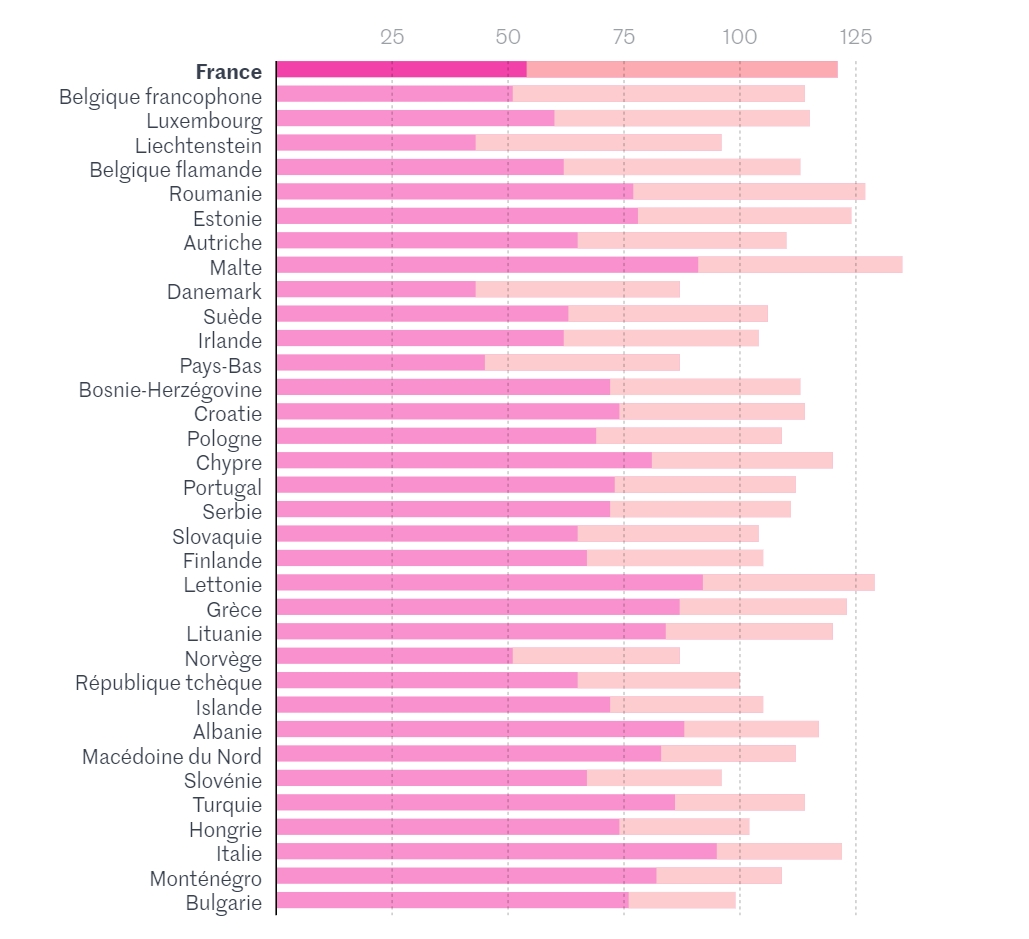
\includegraphics[width=0.9\textwidth]{../Figures/holiday_petites.png}
    \end{figure}
  \end{columns}
\end{frame}

\begin{frame}[label=background2]
  \frametitle{Background: \textit{Vacances Apprenantes} initiatives}
  \begin{figure}
    \centering
    
\includegraphics[width=\textwidth]{../Figures/vacancesapprenantes.png}
  \end{figure}
\end{frame}

% \begin{frame}
%   \frametitle{Background: \textit{Vacances Apprenantes} initiatives}
%   The {program} aims to:
%   \begin{itemize}
%     \item Combat school dropout by maintaining a connection with the school during the
%           crucial period of school holidays and offering a remedial program for students
%           who need it;
%     \item Allow children who cannot go on vacation to benefit from educational, cultural,
%           sports, and outdoor activities;
%     \item Raise young people's awareness of contemporary climate and biodiversity issues
%           through nature discovery activities.
%   \end{itemize}
% \end{frame}

\begin{frame}[label=questions]
  \frametitle{Questions and related literature}
  \alert{Objective}: compare the impact of \textbf{modifying the academic calendar} with \textbf{learning holiday initiatives}.
  \begin{itemize}
    \item Performance measure: academic, physical, mental?
    \item The difference between before and after holiday or the end of year performance?
  \end{itemize}
  \alert{Data}: OECD PISA project across European countries. Survey from the \textit{Vacances apprenantes} program\footnote{which does not exist for the moment.}\\
  \alert{Literature}: mostly in education research. In the US, there are \citet{cooper2003effects, mcmullen2012impact} on the impact of year-round schooling reform. In the UK, \citet{kromydas2022effect,morgan2019socio} studied the impact of summer holiday on inequality, mental health and cognitive ablities.
\end{frame}

\begin{frame}[label=holidaylength]
  \frametitle{Treatment: Length of holiday}
  \alert{Treatment}:
  \begin{itemize}
    \item The length of school holiday is fixed by the education ministry. Everyone has
          to comply. The length varies between countries/regions.
    \item  Policy change from $D=d$ to a set of $D=d'$.
  \end{itemize}
  \alert{Potential outcome}:
  After $D$ days of holiday, the performance $Y_{i}(D)$.\\
  \alert{Treatment effect parameter}: $ATE(X)= E(Y_i(d')-Y_i(d)|X)$.

\end{frame}

\begin{frame}[label=summerschool]
  \frametitle{Treatment: Learning holiday}
  Since this is not compulsory, there will be the usual issue of selection.
  \footnote{To be honest, I am glad that there's selection otherwise I won't able to relate the proposal to the MTE literature.}
  \\
  \alert{Treatment}: "Vacances apprenantes" initiatives.\\
  \alert{Potential outcome}: $Y(1)$ of attending the program.
  $$ Y(1) = \mu_1(X)+U_1$$
  \alert{Choice}: $D=1\{\mu_D(X)>U_D\}$.\\
  \alert{Treatment effect parameter}: MTE (and others)
  \begin{itemize}
    \item $X$ initial performance, family background etc. \footnote{The \href{https://www.aide-sociale.fr/vacances-apprenantes/}{vacances apprenantes} program is targeted at children from disadvantaged backgrounds.}
    \item $Z/X$ the instrument that affects the choice of attending the program, e.g., distance to the summer school camp.
  \end{itemize}
\end{frame}

\begin{frame}
  \frametitle{History}
  \begin{itemize}
    \item "A legacy of the farm economy"?
    \item The rise of urban schools and the need for a break during the hot summer
          months.
    \item A time for leisure, travel, and family bonding.
  \end{itemize}
\end{frame}

%% under 2 different policies, does the $Y_i(0)$ change? 

%% maybe the policy is in effect but some schools are not compiling. Then ?

%% P(Z) represents that given an instrument z, the probability of going to school d2 days. 

%% aaa okay. there's seems to be nothing unusual...

% \begin{frame}
%   \frametitle{MTE?}
%   \textbf{Failed} attempt to link it to the MTE literature:
%   \begin{itemize}
%     \item Continuous instrument $Z$ and $P(Z)$
%     \item Policy Relevant TE: a change from $a \to a'$ corresponds to a change in $P_a(Z)
%             \to P_a'(Z)$.
%   \end{itemize}
%   But if we have $D$ exogenously assigned...? What's the point?
% \end{frame}
% \begin{frame}
%   \frametitle{Questions}
%   \begin{itemize}\itemsep=12pt
%     \item Out of the top 20\% hospitals in France in terms of labor employment
%           efficiency, how many of them are public hospitals/private hospitals?
%     \item What would be the selection outcome if I want to control the number of mistakes
%           that I make?
%     \item Does different selection rule produce different results? And to what degree?
%   \end{itemize}
% \end{frame}

% \section{Data}

% \begin{frame}
%   \frametitle{Hospital Types}
%   The Annual Statistics of Health
%   Establishments
%   (SAE)\footnote{\href{https://data.drees.solidarites-sante.gouv.fr/explore/dataset/708_bases-statistiques-sae/information/}{La
%       Statistique annuelle des établissements (SAE)}}, 2013-2022 \footnote{2020 missing due to Covid-19}.
%   \begin{table}

%     \begin{adjustbox}{width=0.8\textwidth,center}
%       \centering
%       \input{}
%     \end{adjustbox}
%     % \begin{itemize}\itemsep = 8pt
%     %   \item Teaching hospitals may be innately very different from others (training,
%     %         research). \\ \hyperlink{reg_sep}{\beamergotobutton{Appendix}}
%     % \end{itemize}
%   \end{table}
% \end{frame}

% \begin{frame}[label=output]
%   \frametitle{Output}
%   \begin{table}
%     \begin{adjustbox}{width=0.9\textwidth,center}
%       \centering
%       \input{../../Tables/Descriptive/output_share_nonweighted.tex}
%     \end{adjustbox}
%   \end{table}
%   \note{Each value $a_{ij}$ is calculated by $a_{ij} = \frac{\text{Output i only in hospital type j}}{\text{Share of hospital type j}}/\text{Sum of output i}$}

% \end{frame}

% \section{Compound decision and Empirical Bayes}

% \begin{frame}
%   \frametitle{Compound Decision Framework}
%   Observe:
%   \begin{align*}
%     \boldsymbol{\hat{\theta}} & =  (\hat{\theta}_1,\ldots, \hat{\theta}_n)  \\
%     \text{where} \quad        & \hat{\theta}_i | \theta_i \sim P_{\theta_i}
%   \end{align*}
%   Decision:
%   \begin{equation*}
%     \delta(\boldsymbol{\hat{\theta}}) = (\delta_1(\boldsymbol{\hat{\theta}}), \ldots, \delta_n(\boldsymbol{\hat{\theta}}))
%   \end{equation*}
% \end{frame}

% \begin{frame}
%   \frametitle{Compound Loss and Risk}
%   Loss:
%   \begin{equation*}
%     L_n(\theta, \delta(\boldsymbol{\hat{\theta}})) = \sum_{i=1}^n L(\theta_i, \delta_i(\hat{\theta})).
%   \end{equation*}
%   Risk (Expectation of loss):
%   \begin{align*}
%     R_n(\theta, \delta(\boldsymbol{\hat{\theta}})) & = \E[L_n(\theta, \delta(\boldsymbol{\hat{\theta}}))]                                                                                                          \\
%                                                    & = \frac{1}{n}\sum_{i=1}^n \E_{\theta_i|\hat{\theta}_i}[L(\theta_i, \delta_i(\boldsymbol{\hat{\theta}}))]         \quad \text{Separable decision rule } \delta \\
%                                                    & = \frac{1}{n}\sum_{i=1}^n \int L(\theta_i, \delta_i(\hat{\theta}_i))dP_{\theta_i}(\hat{\theta}_i)                                                             \\
%                                                    & = \int \int L(\theta_i, \delta(\hat{\theta}_i))dP_{\theta_i}(\hat{\theta}_i)dG_n(\theta)
%   \end{align*}
%   where $G_n(\theta)$ is the empirical distribution (Frequentist View)\note{$E_{G_n}(f(x)) = 1/n \sum_i f(x_i)$} of $\theta \sim G$.
%   \\$\rightarrow$ Bayesian view: replace $G_n$ by a distribution $G$. $\rightarrow$ Empirical Bayes: Estimate the $G$.
% \end{frame}

% \begin{frame}[fragile]\frametitle{Estimate $G$}
%   \citet{kiefer1956consistency} established the nonparametric maximum likelihood estimator (NPMLE)
%   \begin{equation*}
%     \hat{G}=\argmin_{G\in \mathcal{G}} \set{-\sum_{i=1}^{n}\log g(\hat{\theta}_i)\bigg | g(\hat{\theta}_i)=\int  \p(\hat{\theta}_i |\theta)dG(\theta) }
%   \end{equation*}
%   where $\p(\hat{\theta}_i |\theta)$ is the probability density function of $\hat{\theta}_i$ conditional on the true parameter $\theta$ $\longrightarrow$ $g(\hat{\theta}_i)$ is the marginal pdf of $\hat{\theta}_i$.
% \end{frame}

% \begin{frame}[fragile]{Estimate $G$}
%   This is an \textbf{infinite-dimensional} convex optimization problem with a strictly convex objective subject to linear constraints.
%   \begin{equation*}
%     \min_{f=dG}\set{-\sum_i \log g(y_i)\bigg |g(y_i) = T(f),\ K(f)=1,\ \forall i }
%   \end{equation*}
%   where $ T(f)=\int \p(y_i |\theta)f d\theta $ and  $K(f)= \int f d\theta$.\\

%   Consistency is proven by \citet{kiefer1956consistency}. Efficient computation
%   method introduced by \citet{koenker2014convex}. Implemented with \verb+MOSEK+
%   created by \citet{andersen2010mosek}.
% \end{frame}

% \begin{frame}
%   \frametitle{The Selection Task}
%   \begin{itemize}\itemsep=12pt
%     \item Select the bottom 20\% (the smaller the $\theta_i$, the more efficient) of the
%           true $\theta_i$. Since we assume that $\theta_i \sim G$, those $i$ whose
%           $\theta_i<G^{-1}(0.2)$
%     \item Control the overall false discovery rate at 20\%,
%           \begin{equation*}
%             \frac{\E_G\bra{1\set{\theta_i>\theta_{\alpha},\delta_i=1}}}{\E_G\bra{\delta_i}} \le \gamma
%           \end{equation*}
%           \begin{enumerate}
%             \item Nominator: Selected but whose true value $>G^{-1}(0.2)$.
%             \item Denominator: Selected.
%           \end{enumerate}
%   \end{itemize}
% \end{frame}

% \begin{frame}
%   \frametitle{Problem Formulation}
%   The \textbf{loss} function is
%   \begin{equation*}
%     L(\delta,\theta)=\sum h_i(1-\delta_i) +\tau_1\pa{\sum (1-h_i)\delta_i -\gamma \delta_i} + \tau_2 \pa{\sum \delta_i -\alpha n}
%   \end{equation*} where $h_i=1\set{\theta_i<\theta_{\alpha}=G^-1(\alpha)}$. $h_i$ is an indicator of whether the true value belong to the set. $\delta_i$ is an indicator of whether $i$ is being selected.
%   Therefore, the \textbf{problem} is to find $\delta$ such that
%   \begin{align*}
%     \min_{\delta} \quad & \E_G\E_{\theta|\hat{\theta}}\bra{L(\delta,\theta)}                                                                                                       \\
%     =                   & \E_G \ \sum \E(h_i)(1-\delta_i) +\tau_1\pa{\sum (1-\E(h_i))\delta_i -\gamma \delta_i}                                                                    \\
%                         & + \tau_2 \pa{\sum \delta_i -\alpha n}                                                                                                                    \\
%     =                   & \E_G{\sum v_\alpha(\hat{\theta})(1-\delta_i) +\tau_1\pa{\sum (1-v_\alpha(\hat{\theta}))\delta_i -\gamma \delta_i} + \tau_2 \pa{\sum \delta_i -\alpha n}}
%   \end{align*}
%   where $v_\alpha(\hat{\theta})=\p(\theta<\theta_\alpha|\hat{\theta})$ is the \textbf{posterior tail probability}.
% \end{frame}

% \begin{frame}[label=observation]
%   \frametitle{Derive tail probability $v_\alpha$}
%   Pick hospital $i$ whose true inefficiency value is $\theta_i$, which we don't observe. We only observe a sequence of $Y_{it}$ where
%   \begin{equation*}
%     Y_{it} = \theta_i + \varepsilon_{it} \quad \varepsilon_{it} \sim \caln(0,\sigma_i^2) \quad (\theta_i,\sigma_i^2) \sim G
%   \end{equation*}
%   Neither $\theta_i$ nor $\sigma_i^2$ is known. But the sufficient statistics are
%   \begin{align*}
%     Y_i=\frac{1}{T_i}\sum_{t=1}^{T_i}Y_{it}           & \quad \text{where}\quad Y_i|\theta_i,\sigma_i^2 \sim \caln(\theta_i,\sigma_i^2/T_i)     \\
%     S_i=\frac{1}{T_i-1}\sum_{t=1}^{T_i}(Y_{it}-Y_i)^2 & \quad \text{where} \quad S_i|\sigma_i^2 \sim \Gamma(r_i= (T_i-1)/2,2\sigma_i^2/(T_i-1))
%   \end{align*}
%   In our input demand function specification, we have $Y_{it}=\log(x_{it})-\beta\log(y_{it})$. \hyperlink{normality}{\beamergotobutton{Appendix}}
% \end{frame}

% \begin{frame}
%   \frametitle{TP and Constraints}
%   Given the two sufficient statistics, the posterior tail probability is
%   \begin{align*}
%     v_\alpha(\hat{\theta}_i) & =v_\alpha(Y_i,S_i)                                                                                                         \\
%                              & = P( \theta_i < \theta_{\alpha} | Y_i,S_i)                                                                                 \\
%                              & = \frac{{\int_{-\infty}^{\theta_{\alpha}} \Gamma(s_i|r_i,\sigma_i^2) f(y_i|\theta_i, \sigma_i^2) dG(\theta_i,\sigma_i^2)}}
%     {{\int_{-\infty}^{\infty} \Gamma(s_i|r_i,\sigma_i^2) f(y_i|\theta_i, \sigma_i^2) dG(\theta_i,\sigma_i^2)}}
%   \end{align*}
%   We want to find a cutoff $\lambda$ such that both constraints are satisfied \footnote{Relaxed discrete optimization problem, following \citep{basu2018weighted}}:\\
%   \begin{itemize}\itemsep=8pt
%     \item Capacity: $\int \int P(v_\alpha(Y_i, S_i) > \lambda) dG(\theta_i,\sigma_i^2)
%             \leq \alpha$
%     \item FDR: $\int \int
%             \frac{E[1\{v_\alpha(Y_i,S_i)>\lambda\}(1-v_\alpha(Y_i,S_i))]}{E[1\{v_\alpha(Y_i,S_i)>\lambda\}]}
%             dG(\theta_i,\sigma_i^2) \leq \gamma$
%   \end{itemize}
% \end{frame}

% \begin{frame}{Recap}

%   \begin{enumerate}
%     \item We have a $N\times T$ panel. $Y_{it}$ is an observation of hospital $i$'s
%           inefficiency term $\theta_i$ at time $t$. Say $Y_{it}|\theta_i,\sigma_i \sim
%             \caln(\theta_i,\sigma_i^2)$.
%     \item Given a panel of $Y_{it}$, perform NPMLE to get an estimate of
%           $G(\theta,\sigma^2)$.
%     \item Given the estimated prior $G$, derive the explicit form of posterior tail
%           probability $v_\alpha(Y_i,S_i)$ and the two constraints.
%     \item Solve the selection problem and find the optimal $\delta^*$
%           \begin{equation*}
%             \min_{\delta}\E_G{\sum v_\alpha(\hat{\theta})(1-\delta_i) +\tau_1\pa{\sum (1-v_\alpha(\hat{\theta}))\delta_i -\gamma \delta_i} + \tau_2 \pa{\sum \delta_i -\alpha n}}
%           \end{equation*}
%     \item The decision rule is defined by the cutoff $\lambda^*$
%           \[\delta^*(y_i,s_i)=1\set{v_\alpha(y_i,s_i)>\lambda^*}\]
%   \end{enumerate}
% \end{frame}

% \begin{frame}
%   \frametitle{The estimated $\hat{G}$}
%   \begin{columns}[T,onlytextwidth]
%     \column{0.5\textwidth}
%     Case 1: $G(\theta,\sigma^2)$ for $v_\alpha(Y_i,S_i)$
%     \begin{figure}
%       \centering
%       \includegraphics[width=\textwidth]{../../Figures/2013-2022/GMM_fd/GLVmix.pdf}
%     \end{figure}

%     \column{0.5\textwidth}
%     Case 2: $G(\theta)$ for $v_\alpha(Y_i)$
%     \begin{figure}
%       \centering
%       \includegraphics[width=0.9\textwidth]{../../Figures/2013-2022/GMM_fd/GLmix.pdf}
%     \end{figure}
%   \end{columns}
% \end{frame}

% \begin{frame}
%   \frametitle{The estimated $\hat{G}$}
%   \begin{columns}[T,onlytextwidth]
%     \column{0.5\textwidth}
%     Case 1: $G(\theta,\sigma^2)$ for $v_\alpha(Y_i,S_i)$
%     \begin{figure}
%       \centering
%       \includegraphics[width=\textwidth]{../../Figures/2013-2022/GMM_fd/GLVmix_s.pdf}
%     \end{figure}

%     \column{0.5\textwidth}
%     Case 2: $G(\theta)$ for $v_\alpha(Y_i)$
%     \begin{figure}
%       \centering
%       \includegraphics[width=0.9\textwidth]{../../Figures/2013-2022/GMM_fd/GLmix_s.pdf}
%     \end{figure}
%   \end{columns}
% \end{frame}

% \begin{frame}
%   \frametitle{$G(\theta,\sigma^2)$: Posterior Tail probability (0.2,0.2)}
%   \begin{figure}
%     \centering
%     \includegraphics[width=0.9\textwidth]{../../Figures/2013-2022/GMM_fd/GLVmix/Left_0.2_0.2_TPKWs.pdf}
%   \end{figure}
% \end{frame}

% \begin{frame}
%   \frametitle{$G(\theta)$: Posterior Tail probability (0.2,0.2)}
%   \begin{figure}
%     \centering
%     \includegraphics[width=0.9\textwidth]{../../Figures/2013-2022/GMM_fd/GLmix/Left_0.2_0.2_TPKWs.pdf}
%   \end{figure}
% \end{frame}

% \begin{frame}[label=tpselect]
%   \frametitle{$G(\theta)$: Posterior Tail probability (0.2,0.1)}
%   \begin{figure}
%     \centering
%     \includegraphics[width=0.9\textwidth]{../../Figures/2013-2022/GMM_fd/GLmix/Left_0.2_0.1_TPKWs.pdf}
%   \end{figure}
%   \hyperlink{tpcontour}{\beamergotobutton{Next}}
% \end{frame}

% % \begin{frame}
% %   \frametitle{$G(\theta)$: Posterior Mean}
% %   \begin{figure}
% %     \centering
% %     \includegraphics[width=0.9\textwidth]{../../Figures/2013-2022/GMM_fd/GLmix/Left_0.2_0.2_PMKWs.pdf}
% %   \end{figure}
% % \end{frame}

% % \begin{frame}
% %   \frametitle{$G(\theta)$: James-Stein Shrinkage }
% %   \begin{figure}
% %     \centering
% %     \includegraphics[width=0.9\textwidth]{../../Figures/2013-2022/GMM_fd/GLmix/Left_0.2_0.2_JS.pdf}
% %   \end{figure}
% % \end{frame}

% \begin{frame}
%   \frametitle{"Face value"}
%   \begin{figure}
%     \centering
%     \includegraphics[width=0.9\textwidth]{../../Figures/2013-2022/GMM_fd/GLmix/Left_0.2_0.2_MLE.pdf}
%   \end{figure}
% \end{frame}

% \section{Estimation}
% \begin{frame}{Fixed effect estimation}
%   Assume that $\E[\varepsilon_{it}|\theta_i,x_{i1},\ldots,x_{i,t-1}]=0$.\\
%   \textbf{First Difference GMM}: use lagged level as instruments for current difference
%   \begin{equation*}
%     \E[x_{i,t-2}(\Delta y_{it}-\beta \Delta x_{it})]
%   \end{equation*}
%   System GMM: use lagged difference as instruments for current levels
%   \begin{equation*}
%     \E[\Delta x_{i,t-1}(y_{it}-\beta x_{it})] \quad \text{if}\quad \E\bra{\Delta x_{i,t-1}(\theta_i+\varepsilon_{i,t})}=0
%   \end{equation*}
% \end{frame}

% \begin{frame}
%   \frametitle{Results}
%   \begin{table}\fontsize{6pt}{6pt}\selectfont
%     \input{../../Tables/2013-2022/reg_wg_fd_gmm_c.tex}
%   \end{table}
% \end{frame}

% \section{Conclusion}

% \begin{frame}{Conclusion}
%   \begin{itemize}
%     \item Whether to control for \textbf{False discovery rate}$\rightarrow$Control for
%           FDR shrinks the selection set.
%     \item Whether to assume known $\sigma_i$ makes a difference$\rightarrow$ Assume
%           unknown $\sigma_i$ makes the FDR constraints bind, thus less selected than
%           assuming $\sigma_i$ known.
%     \item Private (FP and NP) hospitals are indeed more "efficient"$\rightarrow$ Caution.
%   \end{itemize}
% \end{frame}

% \begin{frame}[label=limitation]{Limitation}
%   \begin{itemize}\itemsep=12pt
%     \item Interpretation of the $\theta_i$: The Schmidt and Sickles/Pitt and Lee models
%           treat all time invariant effects as inefficiency. \citet{greene2005fixed}
%           treats time invariant components as only unobserved heterogeneity.
%     \item Specification, endogeneity, normality assumption on
%           $\varepsilon_{it}$.\textit{etc.} \hyperlink{normality}{\beamergotobutton{Next}} \end{itemize}
% \end{frame}

\begin{frame}{Thanks!}
  \begin{figure}
    \centering
    
\includegraphics[height=0.5\textwidth]{../Figures/grandesvacanes.jpg}
    % \caption{}
  \end{figure}
\end{frame}

\begin{frame}[allowframebreaks]
  \frametitle{References}
  \bibliography{ref.bib}
  \bibliographystyle{apalike}
\end{frame}

% \appendix

% \begin{frame}[label=inputdemand]{Conditional Input Demand Function}
%   In standard microeconomics, the profit maximization problem is
%   \begin{equation*}
%     \max_{\vec{y}} \sum k_i y_i - \sum p_i x_i \quad \text{subject to} \quad f_i(x_1, x_2, \ldots, x_n) = y_i
%   \end{equation*}
%   where $p_i$ is the price of input $i$ and $f$ is the cost function.

%   The cost minimization problem is thus
%   \begin{equation*}
%     \min_{\vec{x}} \sum p_i x_i \quad \text{subject to} \quad f_i(x_1, x_2, \ldots, x_n) = y_i
%   \end{equation*}
%   Thus, the factor demand function/correspondence is
%   \begin{equation*}
%     x_i = x_i(p_1, p_2, \ldots, p_n, y_1, y_2, \ldots, y_m)
%   \end{equation*}
%   \hyperlink{literature}{\beamergotobutton{Back}}
% \end{frame}

% \begin{frame}[label=production]{Input demand function vs Production function}
%   \begin{itemize}
%     \item We can remain agnostic as to the nature of the appropriate formula for the
%           aggregation of outputs and use as many different products as desired.
%     \item When input prices have low variability. Conditional factor demand can be
%           estimated without information on input prices. Even if we add prices, due a
%           lack of variability, the price parameters will be poorly estimated.

%     \item From $x_i = x_i(p_1, p_2, \ldots, p_n, y_1, y_2, \ldots, y_m)$, we do not need
%           to observe a complete list of inputs. But we do need to observe all input
%           prices (can be ignored if almost no variability) and all outputs. While in the
%           production function, it is the other way around (need to observe all inputs).
%           Since, in our case, output is more \textit{observable} than input (because
%           capital is not easily observed), this approach is preferred.
%   \end{itemize}
% \end{frame}

% \begin{frame}
%   \frametitle{First glance}
%   \begin{columns}[T,T]
%     \column{0.5\textwidth}
%     \makebox[\textwidth][c]{
%       \fontsize{5pt}{5pt} \selectfont
%       \input{../../Tables/2013-2022/reg_pool_iv_ex.tex}}

%     \column{0.5\textwidth}
%     \makebox[\textwidth][c]{
%       \fontsize{5pt}{5pt} \selectfont
%       \input{../../Tables/2013-2022/reg_dummy_iv_ex.tex}}

%   \end{columns}
% \end{frame}

% \begin{frame}[label=reg_sep]{Second glance}
%   \begin{table}
%     \fontsize{6pt}{6pt}\selectfont
%     \input{../../Tables/2013-2022/reg_sep_iv.tex}
%   \end{table}
%   \hyperlink{output}{\beamergotobutton{Back}}
% \end{frame}

% \begin{frame}
%   \frametitle{Panel data Estimator}
%   \begin{itemize}\itemsep=12pt
%     \item Strict exogeneity: Within Group/First Diffrence
%           \begin{equation*}
%             E[\epsilon_{it}|x_{i1},\ldots, x_{iT},\theta_i]=0
%           \end{equation*}
%     \item Relaxed: First Difference GMM \citep{arellano1991some}, System GMM
%           \citep{arellano1995another,blundell1998initial}.
%           \begin{equation*}
%             E[\epsilon_{it}|x_{i1},\ldots, x_{it-p},\theta_i]=0
%           \end{equation*}
%   \end{itemize}

%   Issues: Weak instruments \citep{blundell1998initial} and the proliferation of
%   instruments \citep{roodman2007short}.
%   \begin{equation*}
%     \E[\Delta x_{i,t-1}(y_{it}-\beta x_{it})] \quad \text{if}\quad \E\bra{\Delta x_{i,t-1}(\theta_i+\varepsilon_{i,t})}=0
%   \end{equation*}
% \end{frame}

% \begin{frame}
%   \frametitle{NPMLE Computation Methods}

%   The primal problem:
%   \begin{equation*}
%     \min_{f=dG}\set{-\sum_i \log g(y_i)\bigg |g(y_i) = T(f),\ K(f)=1,\ \forall i }
%   \end{equation*}
%   where $ T(f)=\int p(y_i |\theta)fd\theta $ and  $K(f)= \int f d\theta$.\\
%   Discretize the support:
%   \begin{equation*}
%     \min_{f=dG}\left\{-\sum_i \log g(y_i)\bigg |g=Af,\ {1^T}f=1\right\}
%   \end{equation*}
%   where $A_{ij}= p(y_i|\theta_j) $ and $ f = (f(\theta_1),f(\theta_2),\ldots,f(\theta_m))$.\\
%   The dual problem:
%   \begin{equation*}
%     \max_{\lambda,\mu} \left\{ \sum_i \log \lambda_1(i) \bigg| A^T\lambda_1 < \lambda_2 1,\ (\lambda_1>0) \right\}
%   \end{equation*}
% \end{frame}

% \begin{frame}[label=normality]{Normality assumption on $\varepsilon_{it}$}
%   Estimate the fixed effect $\theta_i$ by
%   \begin{align*}
%     \hat{\theta}_i =                       & \frac{1}{T}\sum(\theta_i+\varepsilon_{it}+x_{it}(\beta-\hat{\beta})) \\
%     \overset{N\to \infty}{\longrightarrow} & \theta_i+\frac{1}{T}\sum_t \varepsilon_{it}
%   \end{align*}
%   When $T$ is relatively small (or even fixed), can't use central limit theorem to claim that $\hat{\theta}_i \overset{d}{\to} \caln(\theta_i,\frac{\sigma_i^2}{T})$.
%   $\longrightarrow$ Assume that $\varepsilon_{it} \sim \caln(0,\sigma_i^2)$ .
%   \hyperlink{observation}{\beamergotobutton{Back (main)}}   \hyperlink{limitation}{\beamergotobutton{Back (end)}}
% \end{frame}

% \begin{frame}
%   \frametitle{$G(\theta,\sigma)$: Posterior Mean}
%   \begin{figure}
%     \centering
%     \includegraphics[width=0.9\textwidth]{../../Figures/2013-2022/GMM_fd/GLVmix/Left_0.2_0.2_PMKWs.pdf}
%   \end{figure}
% \end{frame}

% \begin{frame}
%   \frametitle{$G(\theta,\sigma)$: James-Stein Shrinkage}
%   \begin{figure}
%     \centering
%     \includegraphics[width=0.9\textwidth]{../../Figures/2013-2022/GMM_fd/GLVmix/Left_0.2_0.2_JS.pdf}
%   \end{figure}
% \end{frame}

% \begin{frame}[label=tpcontour]{TP vs PM}
%   \begin{figure}
%     \centering
%     \includegraphics[width=0.9\textwidth]{../../Figures/2013-2022/GMM_fd/GLmix/Contour_Left_0.2_0.1_TPKWs_PMKWs.pdf}
%   \end{figure}
%   \hyperlink{tpselect}{\beamergotobutton{Back}}
% \end{frame}

% \begin{frame}{TP vs JS}
%   \begin{figure}
%     \centering
%     \includegraphics[width=0.9\textwidth]{../../Figures/2013-2022/GMM_fd/GLmix/Contour_Left_0.2_0.1_TPKWs_JS.pdf}
%   \end{figure}
% \end{frame}

% \begin{frame}{TP vs MLE}
%   \begin{figure}
%     \centering
%     \includegraphics[width=0.9\textwidth]{../../Figures/2013-2022/GMM_fd/GLmix/Contour_Left_0.2_0.1_TPKWs_MLE.pdf}
%   \end{figure}
% \end{frame}

\end{document}
